% !TEX root = ACA2019_abstract_pdfgen.tex
% This file should be rename with the speaker's last name. (e.g : smith)

% Write the author names in the order you wish them to appear
% and underline the one who will give the talk.

% Only the speaker's email address is required.

\begin{abstract_online}{Dynamic Applications for Learning and Exploring Mathematics Using Computer Algebra}{%
        \underline{William Bauldr}y$^{1}$, \underline{Wade Ellis}$^{2}$}{[BauldryWC@appstate.edu]
        }{%
        $^1$ Mathematical Sciences, Appalachian State University, Boone, NC. \newline{}
        $^2$ Mathematics Department, West Valley College, Saratoga, California.%
        }
    
%%% Start abstract 
We discuss designing self-contained electronic documents that form a microworld for student investigations; we call these ACR documents. The documents include a CAS application in which students engage in `sandboxed' mathematical exploration. The inquiry-based exploration is led by a set of questions in the document that guide students, experimenting in the computer algebra and dynamic geometry microworlds, that are formulated under the \emph{Action-Consequence-Reflection paradigm}.

The \emph{Action-Consequence-Reflection paradigm} is a research-based pedagogical approach that provides students with a microworld in which to take a mathematical action, observe the consequences of their action, and reflect on the observed behaviour in order to construct mathematical understanding. This paradigm is the basis of the $\Delta\mu$ project which constructed several exemplars and templates for faculty.

We will begin our session with examples of ACR documents, the student exercises/projects that they support, and instructor guides. A screenshot of a sample ACR document is shown in Figure~\ref{fig:ACRDoc1}.
\begin{figure}[!h]
\begin{center}
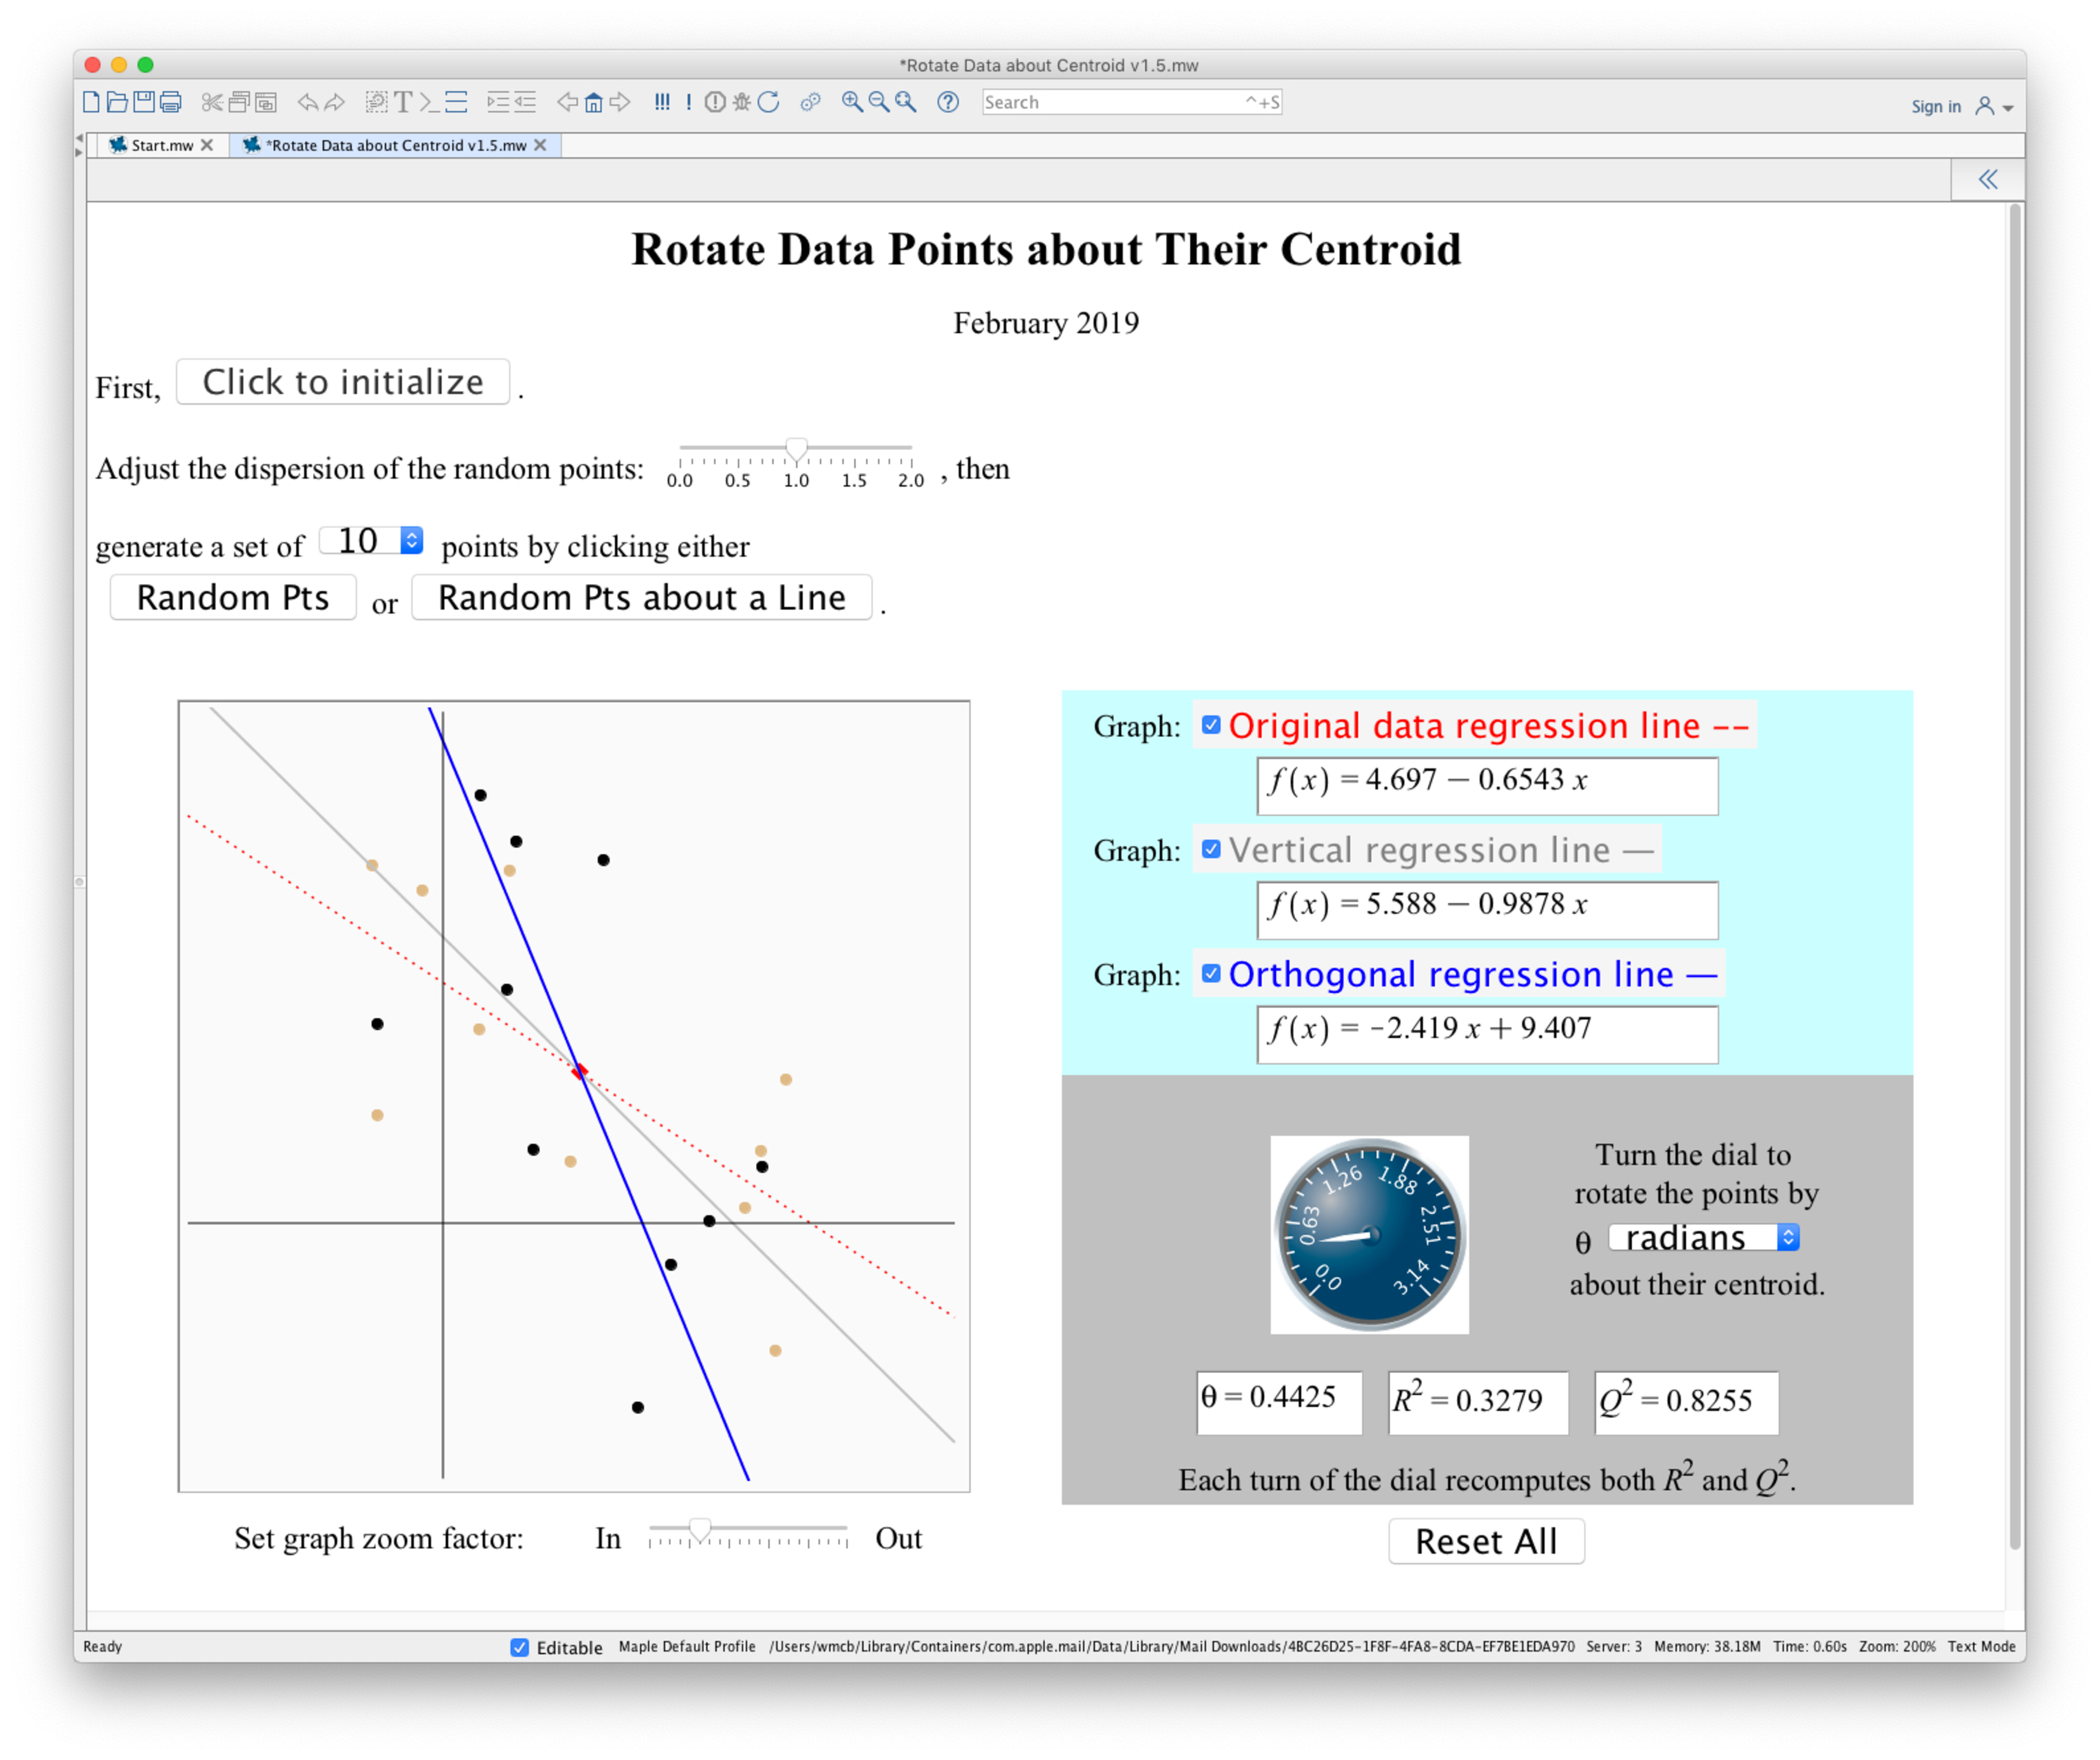
\includegraphics[width=0.65\textwidth]{QSqScreenShot.pdf}
\caption{Linear Regression ACR Maple 2019 Worksheet}
\label{fig:ACRDoc1}
\end{center}
\end{figure}
Then we will move to discussing how to construct ACR documents using Maple 2019 or TI Nspire as our computer algebra substrates. Last, we discuss formulating questions that are the crucial part of the project for students. We'll close with pointers to further information and participant discussion \& questions.
%%% End abstract

\textbf{Keywords} \newline{} 
Dynamic computer algebra pedagogical applications, Action-Consequence-Reflection para- digm

\textbf{References} \newline{}
[1] \textsc{D.~Apple} and \textsc{W.~Ellis}, ``Learning how to learn: Improving the performance of learning,'' Int'l J of Process Education, 7(1), 2015, 21-28.

[2] \textsc{G.~Burrill}, ``The Role of Handheld Technology in Teaching and Learning Secondary School Mathematics,'' ICME 11, TSG-22. Monterrey, M\'{e}xico, 2008.

[3] \textsc{T.~Dick}, \textsc{G.~Burrill}, and \textsc{G.~Brady}, ``New technologies offer new ways to engage students,'' NCSM Newsletter, 38 (2007).

[4] \textsc{W.~Ellis}, ``Technology and Calculus.'' In \emph{Calculus Renewal: Issues for Undergraduate Mathematics Education in the Next Decade}, 53-68, S.~Ganter (ed), Springer US, Boston, 2000.

[5] \textsc{W.~Ellis, W.~Bauldry, M.~Boss\'e,} and \textsc{S, Oteh}, ``Employing Technology to Visualize Complex Roots of Real Polynomials,'' Electronic Proc.~of TIME-2016, UNAM, M\'{e}xico City, Jan.~2017.

[6] \textsc{W.~Bauldry}, ``Using Maple in Modern Algebra and Advanced Calculus Courses,'' Proc. of the 20th Annual ICTCM, 2009, 13-17.

[7] \textsc{E.~Marland}, \textsc{G.~Rhoads}, \textsc{M.~Boss\'e}, \textsc{J.~Sanqui}, and \textsc{W.~Bauldry}, ``$Q^2$: A Measure of Linearity,'' (submitted, Feb., 2019).
\end{abstract_online}
